\chapter{Auswertung der Problematik}\label{chap:problem}
Wie in \autoref{subsec:motivation} bereits beschrieben, liegt der Fokus dieser Arbeit in der Entwicklung einer effizienten und robusten Software-Lösung in Form einer Android-App für die Aufmaßerfassung im Gerüstbau.
Der Prozess der Aufmaßerfassung hat sich im Laufe der Zeit als fehleranfällig und aufwändig herausgestellt.
Im folgenden Kapitel wird am Beispiel der \emph{Fa. VERO} der bisherige, analoge Prozess der Aufmaßerfassung illustriert.
Anschließend wird ein möglicher, optimierter Prozess vorgestellt, der im Verlauf dieser Arbeit mit Hilfe eines IT-Artefakts in Form einer mobilen Applikation für Android-Geräte umgesetzt werden soll.
Bezüglich des \hcdp{} entspricht dieses Kapitel einem Teil der \emph{Observation}.
Die Phase wird erst im nächsten Kapitel vollständig abgeschlossen.

\section{Analyse der Problematik}\label{sec:problem}
In diesem Kapitel wird der charakteristische Vorgang der Aufmaßerfassung im Gerüstbau zunächst beschrieben, und anschließend werden vermeidliche Fehlerquellen, die sich in der Vergangenheit gezeigt haben, evaluiert. \\

Der bisherige Ablauf sieht dabei für einen Monteur der \emph{Fa. VERO} wie folgt aus:
\begin{enumerate}
  \item Fahrt zur Baustelle
  \item Erstellen des Aufmaßes
  \item Aufschreiben der gesammelten Daten auf Papier \label{itm:paper}
  \item Abnahme vom Auftraggeber
  \item Rückfahrt ins Büro
  \item Eintragen der Daten ins System \label{itm:system}
  \item Rechnungsstellung
\end{enumerate}

\noindent
Dieses Verfahren hat sich im Laufe der Zeit als fehleranfällig und zeitaufwändig herausgestellt. 
Durch zu grobe Schätzungen, aber auch die hohe kognitive Belastung der Monteure, kommt es bei der Aufmaßerfassung immer wieder zu Fehlern und damit Kosten, die sich durch eine effizientere Informationsverarbeitung vor Ort auf den Baustellen vermeiden lassen. \\

Insbesondere die Aufgaben in \autoref{itm:paper} bis \autoref{itm:system} des bisherigen Ablaufes sind potentielle Fehlerquellen.
So sind die auf Papier gesammelten Daten (siehe \autoref{fig:notes}) im Nachhinein oft nur vom ursprünglichen Verfasser zu lesen oder gehen noch bevor sie im Büro ins System eingetragen werden können verloren.
Zudem kommt es bei der Nachbearbeitung der Informationen auch häufig dazu, dass Informationen, die vor Ort beim Kunden abgesprochen worden sind, in Vergessenheit geraten und nicht ins System eingetragen werden. \\

Genau diese Problematik soll durch einen optimierten Prozess der Aufmaßerfassung mit Hilfe einer mobilen Applikation für Android-Endgeräte gelöst werden.
Ein solcher optimierter Prozess wird im nächsten Kapitel weiter ausgeführt.

\begin{figure}[h]
  \centering
  \begin{subfigure}[t]{0.4\textwidth}
    \includegraphics[keepaspectratio, width=\textwidth]{aufmasse/front}
    \caption{Gebäudeseite mit Fassadengerüst}
  \end{subfigure}
  \begin{subfigure}[t]{0.4\textwidth}
    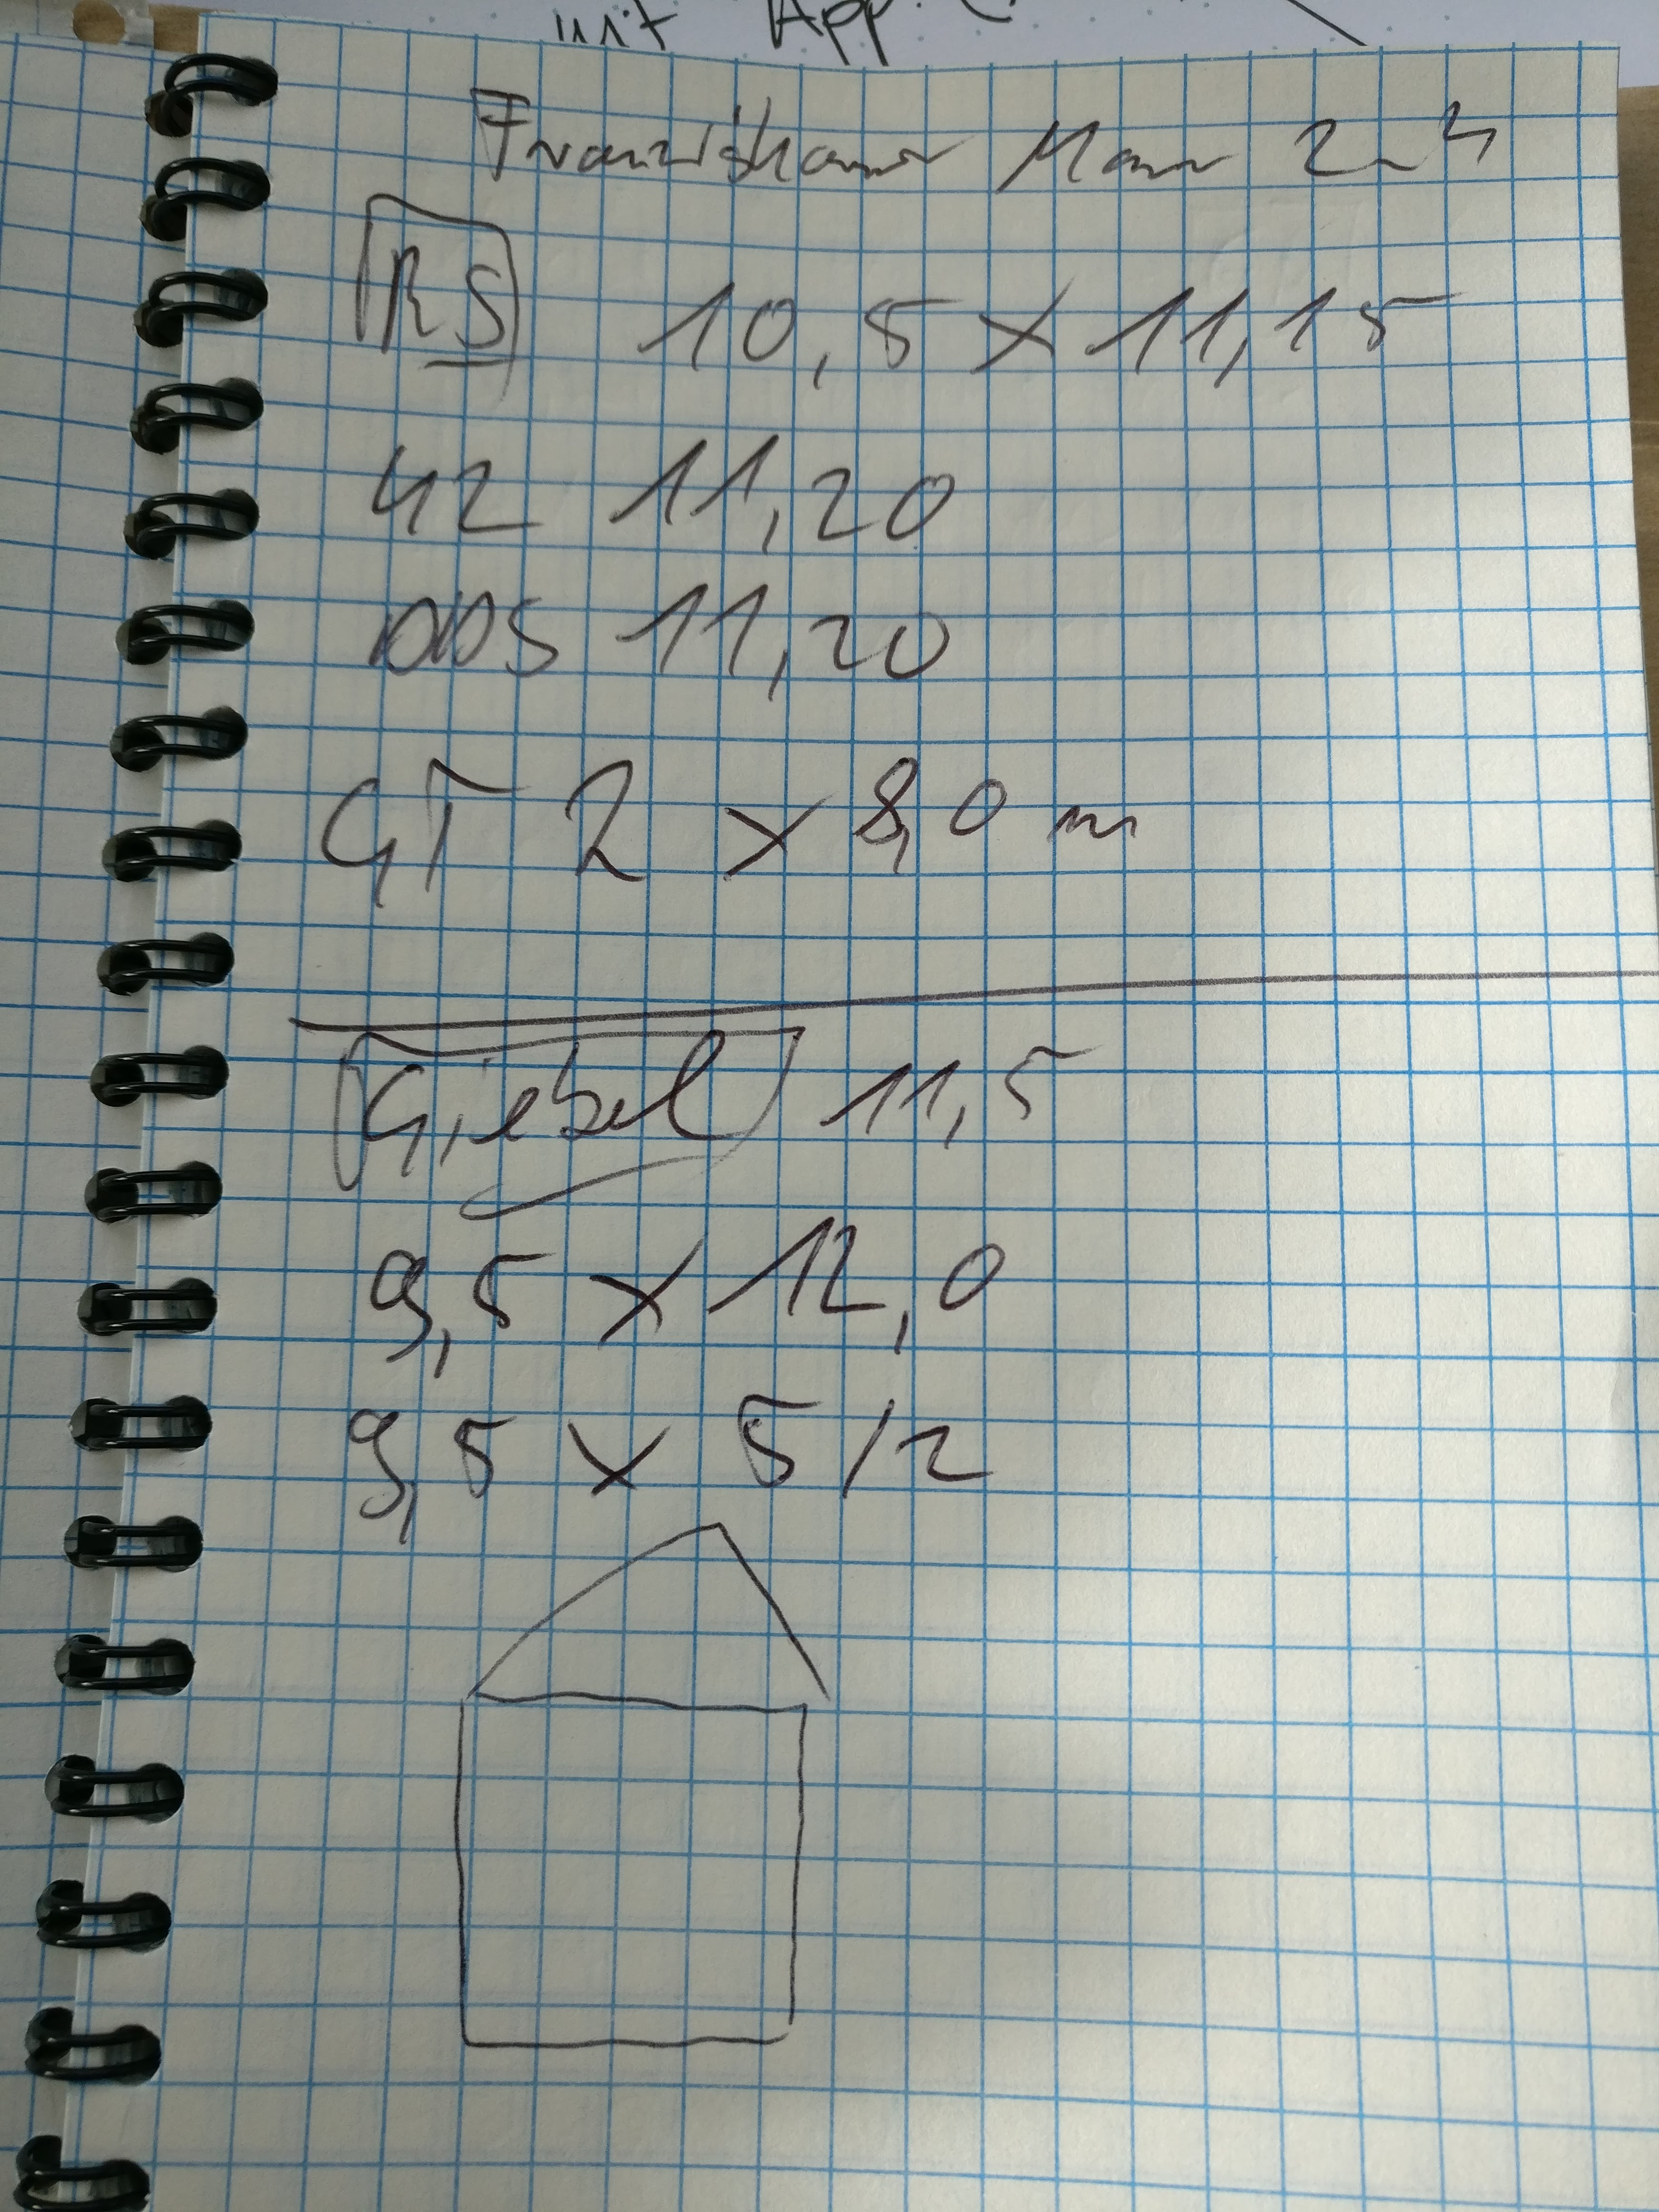
\includegraphics[keepaspectratio, width=\textwidth]{aufmasse/notes}
    \caption{Notizen zum Aufmaß des Fassadengerüsts}
    \label{fig:notes}
  \end{subfigure}
  \caption{Analoge Aufmaßerfassung eines Fassadengerüsts}
  \label{fig:problem}
\end{figure}

In \autoref{fig:problem} sind die Aufmaße eines Fassadengerüst vom X.Y zu sehen.
Diese Notiz stammt aus dem Notizbuch einer der Geschäftsleiter der \emph{Fa. VERO}, der die Aufmaße vor Ort auf der Baustelle angefertigt hat.
\todo{kann ich hier das richtige Datum schreiben, oder machen wir sonst eine Zeitreise?} 

\section{Optimierter Prozess}
Die in \autoref{sec:problem} identifizierten Fehlerquellen ergeben sich durch die hohe kognitive Belastung der Monteure und dem verspäteten Eintragen der gesammelten ggfs. unpräzisen und unvollständigen Informationen ins System erst bei Rückkehr ins Büro. \\

Durch die Entwicklung einer Android-Applikation sollen genau diese Fehlerquellen minimiert und die Effizienz der Monteure gesteigert werden.
Dabei soll die App es dem Benutzer ermöglichen, bereits auf der Baustelle Bilder von den Gerüsten zu machen, die er anschließend mit Hilfe von verschiedenen geometrischen Formen annotieren kann.
Außerdem soll die Möglichkeit bestehen, Informationen wie Länge, Breite und Höhe der Gerüste mit Bezug zum Bild direkt in der App zu hinterlegen. \\

Um den Prozess der Aufmaßerfassung zu vervollständigen, soll es dem Benutzer möglich sein, die annotierten Bilder an einen nachgelagerten Dienst, wie zum Beispiel eine \emph{API}, zu senden.
Die \emph{API} kann anhand der eingetragen Maße ein Aufmaß für den Auftraggeber zur Abnahme generieren.
Ein optimierter Prozess könnte dann beispielsweise wie folgt aussehen:
\begin{enumerate}
  \item Fahrt zur Baustelle
  \item Erstellen der Aufmaße mit Hilfe der App
  \item Abnahme vom Auftraggeber
  \item Rechnungsstellung
\end{enumerate} 

\noindent
Für die Umsetzung einer solchen Lösung stellen sich für den Entwickler verschiedene Fragen, die sich sowohl auf ein positives Anwendererlebnis, als auch auf die robuste Implementierung einer Bearbeitungsumgebung für die aufgenommen Bilder beziehen:

\begin{itemize}
  \item Wie setzt man eine Bearbeitungsumgebung auf dem Smartphone oder Tablet um, die dem Benutzer intuitiv alle möglichen Bearbeitungsoptionen aufzeigt, das Bild dennoch zu jeder Zeit gut erkennbar bleibt?
  \item Auf welche Weise ermöglicht man eine effiziente und zuverlässige Bearbeitungsmethode der aufgenommenen Bilder?
  \item Gibt es spezielle äußerliche Einflüsse, die zu beachten sind, um konstant gute Ergebnisse zu garantieren (Lichtverhältnisse, Aufnahmewinkel)?
  \item Wo liegen eventuelle Grenzen der mobilen Aufmaßerfassung?
  \item Wie lassen sich Meta-Informationen zum Bild (z.B. Beschriftungen von Linien) für eine \emph{API} oder einen nachgelagerten Dienste aufbereiten?
\end{itemize}

\noindent
Wie genau diese Fragen theoretisch, aber auch praktisch umgesetzt werden können, wird in den nachfolgenden Kapiteln weiter ausgeführt.
